\section{\acfp{SNN}}
\label{sec:definitions}

While implementing the \ac{AV} system as a \textit{meta-network} of \acp{SANN}~\cite{sann}, statically analysing it to ensure adherence to the policy $\mathcal{V}_{av}$ would still be extremely difficult due to the usage of \acp{CNN} as the image-processing components of the system and the unknown/unpredictable nature of many of the inputs.
Instead, we propose the usage of \ac{SRE} to ensure system correctness at runtime.
We define the composition of a \ac{SANN} with \ac{SRE} as a \ac{SNN}.

\begin{definition}
	\label{def:ssann}
	An \ac{SNN} is formalised as a tuple $S = \langle I,~O,~\mathcal{V}_I,~\mathcal{V}_O,~L,~\gamma,~\alpha  \rangle$, where:
	\begin{itemize}
		\item $I$ is a finite collection of input variables with
		its domain being $\mathbf{I} = \mathbb{R}^n$.
		\item  $O$ is a finite collection of  output variables with
		its domain being $\mathbf{O} = \mathbb{R}^m$.
		\item $\mathcal{V}_I$ is an input safety policy, defined by a safety automaton~\cite{recps}, specifying the safe behaviour of inputs $I$.
		\item $\mathcal{V}_O$ is an output safety policy, defined by a safety automaton, specifying the safe behaviour of input-outputs $I \times O$.
		\item $L$ denotes a set of \ac{ANN} layers $\{l_i,~l...~,~l_{pp}\}$. Each layer is described by its layer type, starting with the input layer $l_i$ and iterating through the \ac{ANN} until the post-processing layer $l_{pp}$.
		\item $\gamma: I_l \rightarrow O_l$ is the non-linear activation function that provides the behaviour of a given layer, i.e. when provided inputs $I_l$, the layer produces outputs $O_l$.
		\item $\alpha: l_k \rightarrow l_{k+1}$ is the layer-to-layer mapping function that maps the outputs $O$ of each \ac{ANN} layer to the inputs  $I$ of the following layer. $O_k$ maps to $I_{k+1}$ such that every input of layer $k+1$ has at least one output from layer $k$ connected to it. 
	\end{itemize}
\end{definition} 

To run a given \ac{SNN} (i.e. fully complete computation over an input set $\mathbf{I}$), the functions $\gamma$ and $\alpha$ will each need to be called once for every layer (apart from the output layer, on which only $\gamma$ is called).

%\begin{figure}[t]
%	\centering
%	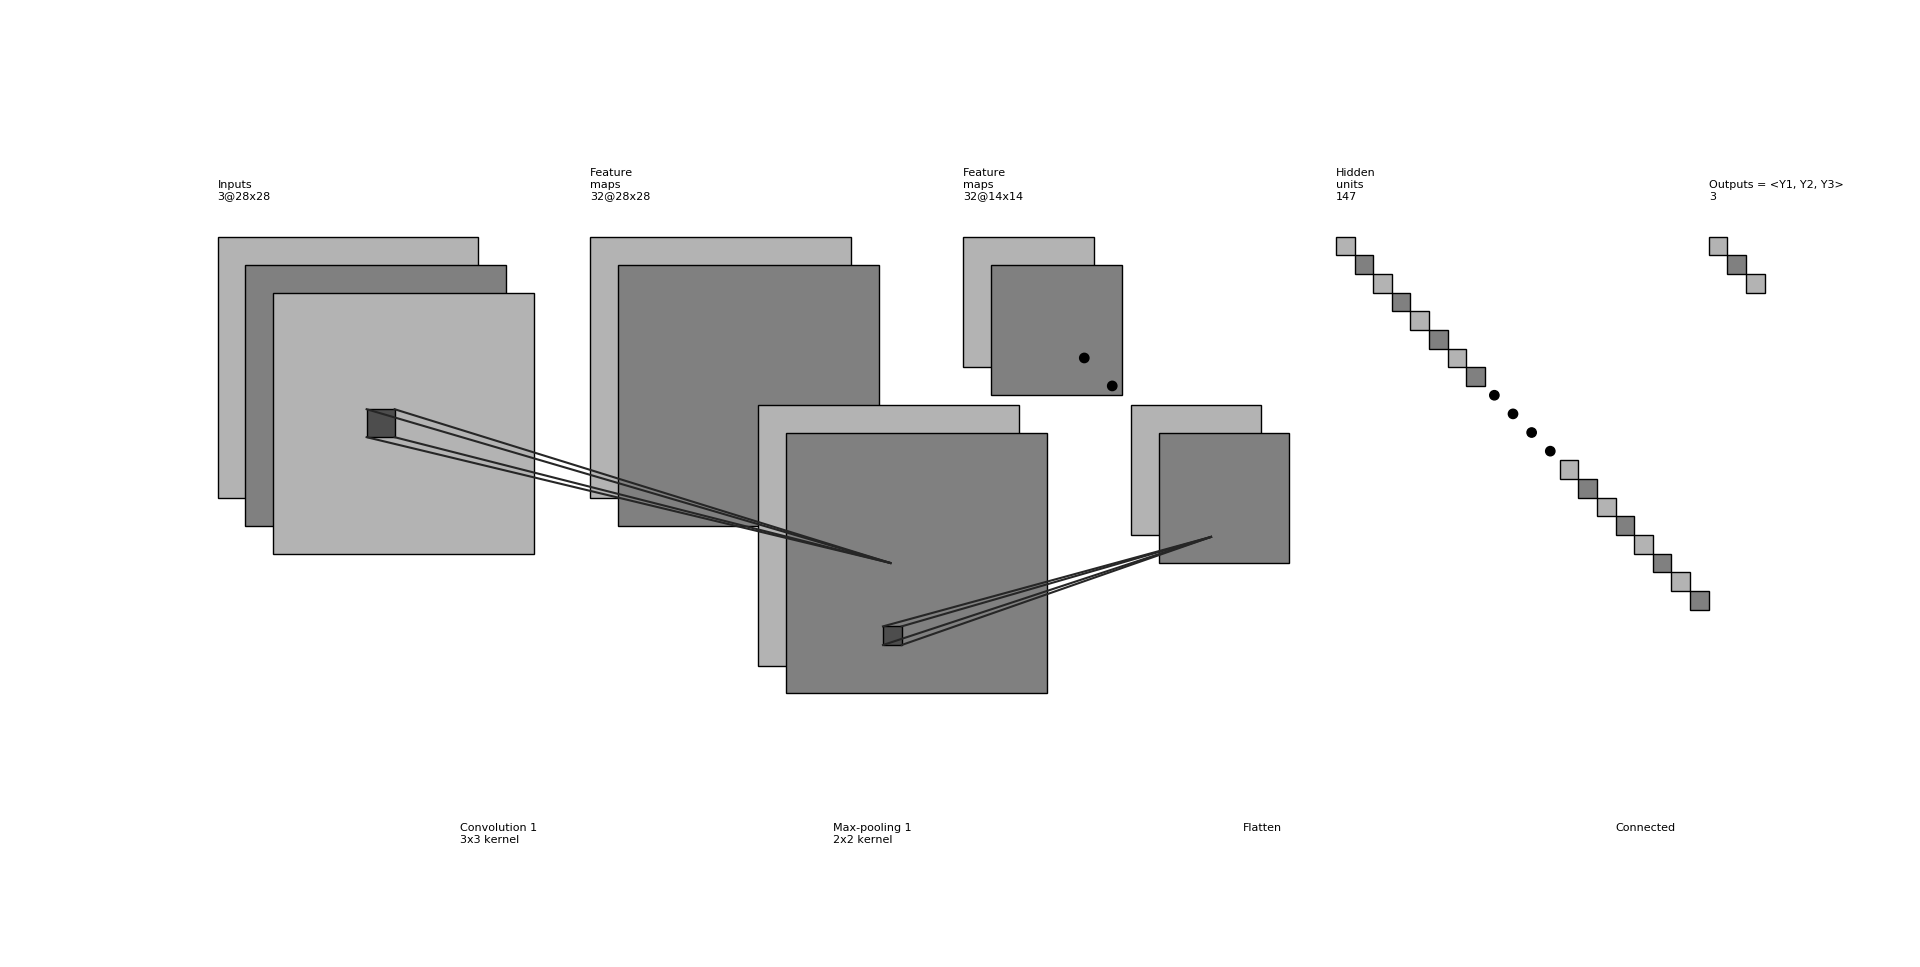
\includegraphics[width=\linewidth]{fig/CNN.png}
%	\caption{Diagram showing the structure of a basic \ac{CNN}.	\label{fig:cnn}}
%\end{figure}

\begin{figure}[b]
	\centering
	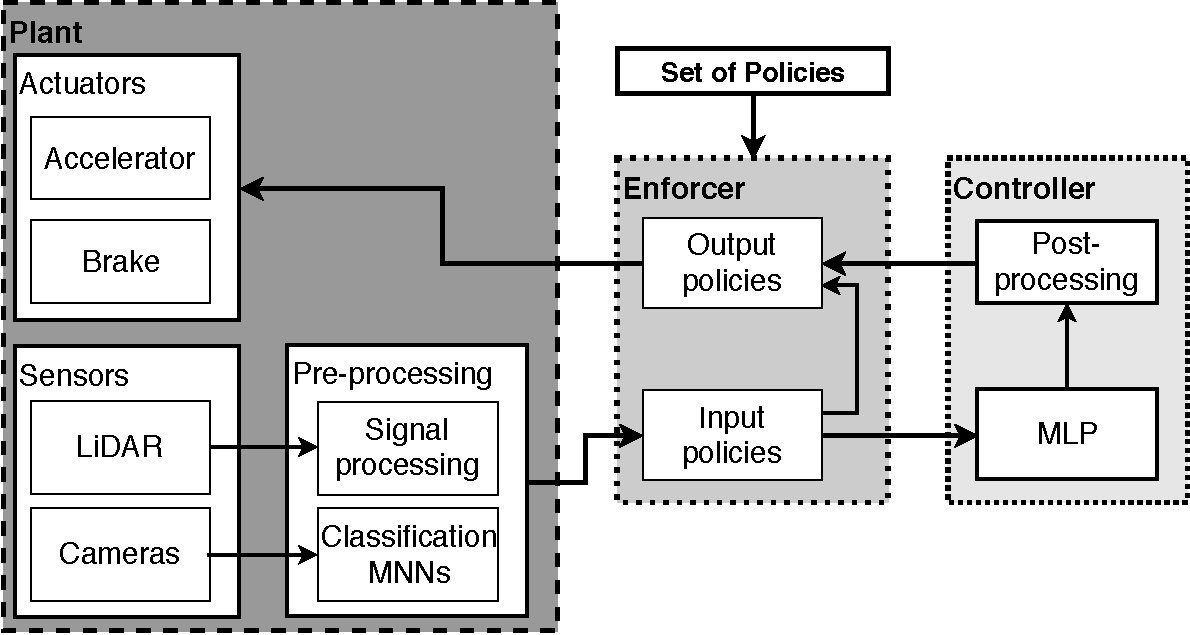
\includegraphics[width=\linewidth]{Content/fig/AV-sys.pdf}
	\caption{Diagram showing the system design for the \ac{AV}. \label{fig:avsys}}
\end{figure}

\subsection{\ac{AV} system as a \ac{SNN}}
%\todo{You have no page limit at the moment so add the other policies to this document so Partha can see them}

The \ac{AV} system described in Section~\ref{sec:case} can be demonstrated as the combination of components and connections shown in Figure~\ref{fig:avsys}.
It can be presented formally using Definition~\ref{def:ssann} with:
\begin{itemize}
	\item $I=\langle S,~P,~O_{1},~O_{1_S},~O_{1_D}...,~O_{5},~O_{5_S},~O_{5_D} \rangle$, i.e. the 17 different fixed-point integer inputs to the controller \ac{ANN} described in Section~\ref{sec:case}.
	\item $O = \langle A, B_S, B_H \rangle$ are the three different fixed-point integer outputs which represent the different actions (and the confidence in the action) that can be taken by the \ac{AV} at any given time.
	\item $\mathcal{V}_I = \mathcal{V}_{av_I} = \mathcal{V}_{cnn_I} \wedge \mathcal{V}_{ped_I} \wedge \mathcal{V}_{car_I} \wedge \mathcal{V}_{drive_I}$, i.e. the complete set of policies projected on inputs $I$. Once combined, they ensure the safety of the \ac{CNN} ensemble and \ac{LiDAR} outputs (i.e. the controller's inputs).
	\item $\mathcal{V}_O = \mathcal{V}_{av} = \mathcal{V}_{cnn} \wedge \mathcal{V}_{ped} \wedge \mathcal{V}_{car} \wedge \mathcal{V}_{drive}$, i.e. the complete set of policies ensuring the safety of the controller. Once combined, they prevent collisions with pedestrians, other vehicles and maintain that the car drives consistently and within the law.
	\item $L = \{l_i,~l_h,~l_o,~l_{pp}\}$, are the four layers of the controller \ac{ANN}, i.e. the input layer, hidden layer, and output layer of the \ac{MLP}; and the post processing layer of the controller.
	%\item The function $\gamma$ given input $\langle I_{h_1}, I_{h_2}, ..., I_{h_17} \rangle$ to the hidden layer $l_h$ produces the output vector $\langle O_{h_1}, O_{h_2}, ..., O_{h_17} \rangle$, i.e. one output for each neuron in the hidden layer. 
	%\item The function $\alpha$ maps one layer's outputs to the next layer's inputs, e.g. the inputs $I_{o}$ of the output layer $l_o$ are derived from the outputs $O_{h}$ of the hidden layer $l_h$ using $I_{o} = \langle \alpha(O_{h}) \rangle = \langle \displaystyle \sum_{j}^{i=1} O_{h_1}.w_{1_i}, \displaystyle \sum_{j}^{i=1} O_{h_2}.w_{2_i}, \displaystyle \sum_{j}^{i=1} O_{h_3}.w_{3_i} \rangle$, where $j$ is the number of neurons in the hidden layer, and $w_{m_n}$ is the hidden layer weight at corresponding to the $m^{th}$ output neuron and the $n^{th}$ hidden layer neuron. 
	%\item \todo{How does the post-processing fit into this definition? It is clearly between the MLP and the output enforcer. You may need to justify post-processing as a fourth layer of the MLP, and change the MLP to some different ANN name. I have attempted to fit this already.} 
\end{itemize}
%The network function $\eta$ given input $\langle 0, 0, ..., 0 \rangle$ produces an output $\langle 1, 0, 0 \rangle$ i.e. $\eta(\langle 0, 0, ..., 0 \rangle) = \langle 1, 0, 0 \rangle$.


The bi-directional enforcer for this system enforces the properties in Section~\ref{sec:case} %$\mathcal{V}_{av}$,
%These can be represented as \ac{DTA}, and then ANDed together to produce a single \ac{DTA}, as seen in Figure~\ref{fig:avrte}. %\todo{Figure 2 doesn't show the full DTA. This is wrong.}
%Each policy is defined by a Safety Automaton, with the pedestrian avoidance policy being a \ac{DTA}.
%The policies are combined by ANDing the states of each policy together to create a single, larger policy that includes each other policy.
%The policy is enforced using a bi-directional runtime enforcer, 
and is seen in the complete system in Figure~\ref{fig:avsys}.

\begin{example}
	Assume the system is in state $l_{drive}$ with the car cruising at 50 km/h.
	Suddenly, a pedestrian steps into the road ahead and to the left of the vehicle.
	Hence, the \ac{SNN} receives an input vector $\mathbf{I}$ describing the environment, including the vehicles current speed and the pedestrian detected on the left-most sensor.% and output a corresponding action.
	The safe reaction would be to slow down and act with caution until the pedestrian has been passed, or brake hard if the pedestrian walks in front of the vehicle.
	
	Since the ensembles correctly identified the pedestrian, and agree with the \ac{LiDAR} readings, the input enforcer $\mathcal{V}_I$ does not modify any of the inputs in $\mathbf{I}$.
	The functions $\gamma$ and $\alpha$ are called on every \ac{ANN} layer except the output layer, where only $\gamma$ is called.
	Suppose the controller \ac{ANN} is in the early stages of training and does not recognise a pedestrian walking to the road as a potential safety hazard, the \ac{ANN} outputs that nothing should be done in this situation (i.e. $\langle 0, 0, 0 \rangle$).
	The output enforcer $\mathcal{V}_O$ recognises that this is not the desired output, and initiates a braking sequence by changing the \ac{ANN} outputs to gently brake (i.e. $\langle 0, 1, 0 \rangle$) and sets the output vector $\mathbf{O}$ to the new \ac{ANN} outputs.
	The braking action, along with the positioning of the pedestrian, causes the enforcer to change to the state $l_{brake}$.
\end{example}

\subsection{Training the \ac{AV} \acp{ANN}}
Since the ideal outputs for the controller are unknown, due to the large number of states the system could be in at any given time, the system could not be trained using standard back-propagation with gradient descent.
Instead, a reinforcement learning algorithm was used for the training phase of the controller.
The algorithm rewarded vehicles that did well during the training, while penalising those that did not.
%Due to the hardware limitations, the system was trained for, at most, 10,000 epochs. 
%At 1, 10, 100, 1,000 and 10,000 epochs the state of the controller \ac{ANN} was saved and used for testing. 
%At each of the trained epochs, the aforementioned policies were enforced, and the resultant behaviour of each \ac{ANN} state was recorded.
%The results of this system are shown in Section~\ref{sec:results}.


%\begin{example}
%	The \ac{AV} system controller \ac{SNN} described in Section~\ref{sec:case} can be presented formally with:
%	\begin{itemize}
%		\item $I=\langle x_1, x_2, ..., x_{2352} \rangle$, i.e. the flattened input of the $28 \times 28 \times 3$ input image. 
%		\item $O = \langle Y_1, Y_2, Y_3 \rangle$.
%		\item $\mathcal{V}_I = \mathcal{V}_{cnn}$, i.e. the policy that modifies the \ac{CNN} ensemble outputs in the case of clashing class confidence values.
%		\item $\mathcal{V}_O = \mathcal{V}_{ped} \wedge \mathcal{V}_{car} \wedge \mathcal{V}_{drive}$, i.e. the policies that prevent collisions with pedestrians, other vehicles and maintain that the car drives consistently and within the law.
%		\item $L = \{Input, Convolution 1, ..., Connected, Output\}$, as described in Figure~\ref{fig:cnn}.
%		\item The function $\gamma$ given input $\langle I_{Maxpooling 1} \rangle$ to layer $Maxpooling 1$ produces the output vector $\langle maxpool(I_{Maxpooling 1}) \rangle$. 
%		\item The function $\alpha$ maps layer outputs to layer inputs, e.g. the inputs $I_{Maxpooling 1}$ of $Maxpooling 1$ are derived from the outputs $O_{Convolution 1}$ of $Convolution 1$ using $I_{Maxpooling 1} = \langle \alpha(O_{Convolution 1}) \rangle = \langle O_{Convolution 1} \rangle$. 
%		\item The network function $\eta$ given input image $\langle \mathbf{I_{image}} \rangle$ produces an output $\langle \mathbf{O} \rangle = \eta(\langle \mathbf{I_{image}} \rangle) = \langle P_1, P_2, ..., P_n \rangle$ where $P_1$ is the probability of the input image being the $1^{st}$ class and $P_n$ is the probability of the input image being the $n^{th}$ class.
%	\end{itemize}
%\end{example}


%\begin{figure}[t]
%	\centering
%	\scalebox{0.9}{\def\layersep{2.25cm}
\begin{tikzpicture}[shorten >=1pt,->,draw=black!100, node distance=\layersep]
	\tikzstyle{every pin edge}=[<-,shorten <=1pt]
	\tikzstyle{neuron}=[circle,fill=black!25,minimum size=20pt,inner sep=0pt]
	\tikzstyle{input neuron}=[neuron, fill=white!100,draw=black];
	\tikzstyle{output neuron}=[neuron, fill=white!100,draw=black];
	\tikzstyle{hidden neuron}=[neuron, fill=white!100,draw=black];
	\tikzstyle{annot} = [text width=4em, text centered]
	
	% Draw the input layer nodes
	\foreach \name / \y in {1,...,2}
	% This is the same as writing \foreach \name / \y in {1/1,2/2,3/3,4/4}
	\node[input neuron, pin=left:Input $x_\y$] (I-\name) at (0,-\y) {$i_\y$};
	
	% Draw the hidden layer nodes
	\foreach \name / \y in {1,...,3}
	\path[yshift=0.5cm]
	node[hidden neuron] (H-\name) at (\layersep,-\y cm) {$h_\y$};
	
	% Draw the output layer node
	\node[output neuron,pin={[pin edge={->}]right:Output $y$}, right of=H-2] (O1) {$o_1$};
	
	% Connect every node in the input layer with every node in the
	% hidden layer.
	%\foreach \source in {1,...,2}
	%\foreach \dest in {1,...,3}
	%\path (I-\source) edge node[above] {1} (H-\dest);
	\path (I-1) edge node[above] {1} (H-1);
	\path (I-1) edge node[above] {0.5} (H-2);
	\path (I-2) edge node[above] {0.5} (H-2);
	\path (I-2) edge node[above] {1} (H-3);
	
	% Connect every node in the hidden layer with the output layer
	%\foreach \source in {1,...,3}
	\path (H-1) edge node[above] {1} (O1);
	\path (H-2) edge node[above] {-2} (O1);
	\path (H-3) edge node[above] {1} (O1);
	
	% Annotate the layers
	\node[annot,above of=H-1, node distance=2cm] (hl) {\textit{Hidden Layer}\\$l_h$};
	\node[annot,left of=hl] {\textit{Input Layer}\\$l_i$};
	\node[annot,right of=hl] {\textit{Output Layer}\\$l_o$};
\end{tikzpicture}}
%	\caption{Example of an \ac{MLP}.	\label{fig:ann}}
%\end{figure}
%\begin{example}
%	Likewise, the \ac{MLP} presented in Figure~\ref{fig:ann} can be presented formally, using the same definition:
%	\begin{itemize}
%		\item $I=\langle x_1, x_2 \rangle$. 
%		\item $L = \{l_i, l_h, l_o\}$. 
%		\item The function $\gamma$ given input $\langle 1, 0.5, 0 \rangle$ to layer $l_h$ produces the output vector $\langle 1, 1, 0 \rangle$. 
%		\item The function $\alpha$ maps layer outputs to layer inputs, e.g. the inputs $I_{lo}$ of $l_o$ are derived from the outputs $O_{lh}$ of $l_h$ using $I_{lo} = \langle \alpha(O_{lh}) \rangle = \langle (O_{lh1} * 1) + (O_{lh2} * -2) + (O_{lh3} * 1) \rangle$. 
%		\item The network function $\eta$ given input $\langle 0, 1 \rangle$ produces an output $1$ i.e. $\eta(\langle 0, 1 \rangle) = 1$.
%	\end{itemize}
%\end{example}
